\documentclass[11pt]{amsart}
\usepackage[margin=1.1in]{geometry}
\usepackage{amssymb,mathtools}
\usepackage{graphicx}
\usepackage[hidelinks]{hyperref}
\usepackage{doi}

\newtheorem{theorem}{Theorem}[section]
\newtheorem{lemma}[theorem]{Lemma}
\newtheorem{proposition}[theorem]{Proposition}
\newtheorem{corollary}[theorem]{Corollary}
\newtheorem*{theoremA}{Theorem A}
\newtheorem*{theoremB}{Theorem B}
\theoremstyle{definition}
\newtheorem{definition}[theorem]{Definition}
\theoremstyle{remark}
\newtheorem{remark}[theorem]{Remark}

\newcommand{\R}{\mathbb{R}}
\newcommand{\cA}{\mathcal{A}}
\DeclareMathOperator{\arcsec}{arcsec}

\begin{document}

\title{Antipodal Chords of Closed Curves and the Exponent Three}

\author{Deep Bhattacharjee}
\address{Formerly, Electro-Gravitational Space Propulsion Laboratory (EGSPL), Bhubaneswar, Odisha 751030, India}
\address{Formerly, University of Calcutta (Heramba Chandra College), 23/49 Gariahat Road, Golpark, Kolkata 700029, West Bengal, India}
\email{d.bhattacharjee@erl-forschung.de}
\email{itsdeep@live.com}
\email{egspl@proton.me (GitHub-related contact; GitHub: creelie)}
\urladdr{https://orcid.org/0000-0003-0466-750X}

\subjclass[2020]{52A40, 53A04, 49K15, 81Q10}
\keywords{mean-chord inequality, isoperimetric problem, antipodal chords, Pontryagin maximum principle, leaky quantum graphs}

\begin{abstract}
For a closed curve of length $L$, the chord joining two points at arclength distance $L/2$ is an antipodal chord. We prove that among all closed curves of length $L$ in $\R^d$ the circle uniquely maximizes the $p$-th mean of the antipodal chord length for every $p\le 3$, and that the circle is not even a local maximizer when $p>3$. This settles the half-length case of the mean-chord problem of Exner, Harrell and Loss, which was known only for $p\le 2$, and shows that the critical exponent there is $3$ and not $5/2$.
\end{abstract}

\maketitle

\section{Introduction}

Let $\Gamma\colon\R\to\R^d$ be a closed rectifiable curve of length $L$, parametrized by arclength, so that $\Gamma$ is $L$-periodic and $|\Gamma'|=1$ almost everywhere. For $0<u<L$ and $p>0$ consider the $p$-th mean of the chords that join points at arclength distance $u$,
\[
c_p(\Gamma,u)=\frac1L\int_0^L|\Gamma(s+u)-\Gamma(s)|^p\,ds .
\]
On the circle of length $L$ every such chord has length $\frac L\pi\sin\frac{\pi u}L$. The question whether
\begin{equation}\label{eq:EHL}
c_p(\Gamma,u)\le\Bigl(\frac L\pi\sin\frac{\pi u}{L}\Bigr)^p
\end{equation}
holds for all closed curves goes back to Lük\H{o} \cite{Luk66}, who proved it for $p=2$; Pech \cite{Pec92} gave another proof in all dimensions. Exner \cite{Exn05} and Exner, Harrell and Loss \cite{EHL06,EHL06a} found that \eqref{eq:EHL} governs two isoperimetric problems in mathematical physics: the shape of a loop of given length that maximizes the ground-state energy of a leaky quantum graph $-\Delta-\alpha\delta(x-\Gamma)$ in the plane, and the equilibrium shape of a uniformly charged loop; see also the review \cite{Exn08}. They proved \eqref{eq:EHL} for every $p\le2$ and asked for the largest exponent for which it remains true. By Jensen's inequality, validity for one exponent implies validity for every smaller one. A stadium shows that \eqref{eq:EHL} fails for $p$ above about $3.15$ \cite{EHL06}, and the numerical experiments of Abrams, Cantarella, Fu, Ghomi and Howard \cite{ACFGH03} point to a threshold between $3.3$ and $3.58$ for the double integral $\iint|\Gamma(s)-\Gamma(t)|^p\,ds\,dt$, which averages \eqref{eq:EHL} over $u$. Exner, Fraas and Harrell \cite{EFH07} studied the second variation of $c_p(\cdot,u)$ at the circle and stated that the circle stops being a local maximizer when $p$ exceeds $(4-\cos\frac{2\pi u}L)/(1-\cos\frac{2\pi u}L)$, a number equal to $5/2$ for $u=L/2$. Beyond $p=2$ no global result has been known for any $u$.

This paper settles the case $u=L/2$ completely. We call $\Gamma(s+L/2)-\Gamma(s)$ an antipodal chord.

\begin{theoremA}
Let $d\ge2$ and let $\Gamma$ be a closed rectifiable curve of length $L$ in $\R^d$. For every $0<p\le3$,
\[
\frac1L\int_0^L\Bigl|\Gamma\Bigl(s+\frac L2\Bigr)-\Gamma(s)\Bigr|^p\,ds\le\Bigl(\frac L\pi\Bigr)^p ,
\]
with equality if and only if $\Gamma$ is a circle traversed once. For every $p>3$ there are smooth closed plane curves of length $L$, arbitrarily close to the circle in $C^\infty$, for which the inequality fails.
\end{theoremA}

The second part of Theorem A comes from an explicit deformation of the circle that works for every $u$.

\begin{theoremB}
For $0<u<L$ and $p>3/\sin^2(\pi u/L)$ there are smooth closed plane curves of length $L$, arbitrarily close to the circle in $C^\infty$, for which \eqref{eq:EHL} fails. For $u=L/2$ the circle is the global maximizer for every $p\le3$.
\end{theoremB}

Since $3/\sin^2(\pi u/L)$ is larger than $(4-\cos\frac{2\pi u}L)/(1-\cos\frac{2\pi u}L)$ for every $u$, Theorem B is consistent with the stability statement of \cite{EFH07} for $p$ below their threshold. For $u=L/2$, however, Theorem A shows that the circle is the global maximizer for all $p$ in $(5/2,3]$, so the assertion of \cite{EFH07} that the circle fails to be a local maximizer for $p>5/2$ is incorrect. The second variation along the deformation used below changes sign exactly at $p=3/\sin^2(\pi u/L)$ (Proposition~\ref{prop:mode2}); this is the mode $n=2$ of \cite{EFH07}, whose coefficient there has the wrong sign between the two thresholds. Figure~\ref{fig:apsidal} compares the two curves.

The proof of Theorem A has three steps. First, half of the antipodal chord is a $1$-Lipschitz loop $W$ that satisfies $W(t+\pi)=-W(t)$ (Section~\ref{sec:reduction}). The problem becomes an optimal control problem: maximize $\int|W|^3$ over such loops. Second, the Pontryagin maximum principle turns a maximizer into an orbit of a central force problem, whose integrals of motion classify the candidates (Sections~\ref{sec:pmp} and~\ref{sec:orbits}). Third, an extremal loop that is neither the circle nor too small to matter would need an apsidal angle equal to an odd multiple of $\pi$, and we show that the apsidal angle lies strictly between $\pi$ and $3\pi$ (Section~\ref{sec:apsidal}). The last step reduces to an explicit polynomial inequality, and it is there that the exponent $3$ enters: for $p=3$ the apsidal angle tends to $\pi$ at both ends of the family of orbits.

\section{Reduction to antipodal loops}\label{sec:reduction}

By scaling we take $L=2\pi$ in Sections~\ref{sec:reduction}--\ref{sec:proofA}. Write $|\cdot|$ for the Euclidean norm on $\R^d$ and
\begin{gather*}
\cA=\bigl\{w\colon[0,\pi]\to\R^d:\ |w(t)-w(t')|\le|t-t'|\ \text{for all }t,t',\ \ w(\pi)=-w(0)\bigr\},\\
J(w)=\int_0^\pi|w(t)|^3\,dt .
\end{gather*}
Every $w\in\cA$ extends to a $2\pi$-periodic $1$-Lipschitz map $W\colon\R\to\R^d$ with $W(t+\pi)=-W(t)$; we use the same letter for a loop and its extension.

\begin{lemma}\label{lem:reduction}
Let $\Gamma$ be a closed curve of length $2\pi$ parametrized by arclength and put $W(s)=\tfrac12\bigl(\Gamma(s+\pi)-\Gamma(s)\bigr)$. Then $W|_{[0,\pi]}\in\cA$ and
\[
\frac1{2\pi}\int_0^{2\pi}|\Gamma(s+\pi)-\Gamma(s)|^3\,ds=\frac8\pi\,J(W).
\]
If $|W'|=1$ almost everywhere, then $\Gamma$ is a translate of $-W$.
\end{lemma}

\begin{proof}
$W(s+\pi)=\frac12(\Gamma(s+2\pi)-\Gamma(s+\pi))=-W(s)$, and $|W'|\le\frac12(|\Gamma'(s+\pi)|+|\Gamma'(s)|)=1$ almost everywhere. The integrand is $8|W|^3$, and $|W|$ is $\pi$-periodic. If $|W'(s)|=1$, the two unit vectors $\Gamma'(s+\pi)$ and $\Gamma'(s)$ are at distance $2$, hence opposite, and $W'(s)=-\Gamma'(s)$.
\end{proof}

Theorem A for $p=3$ is therefore equivalent to $J(w)\le\pi$ on $\cA$, with equality only for unit circles traversed at unit speed. The circle $w(t)=e_1\cos t+e_2\sin t$, with $e_1,e_2$ orthonormal, gives $J=\pi$.

\begin{lemma}\label{lem:zero}
If $w\in\cA$, then $|w|\le\pi/2$. If moreover the extension $W$ vanishes somewhere, then $J(w)\le\pi^4/32<\pi$.
\end{lemma}

\begin{proof}
For $t\in[0,\pi]$, $2|w(t)|\le|w(t)-w(0)|+|w(t)-w(\pi)|\le t+(\pi-t)$. If $W(t_0)=0$, then $W(t_0+\pi)=0$, and $|W(t)|\le\min(t-t_0,\,t_0+\pi-t)$ on $[t_0,t_0+\pi]$. Since $|W|$ is $\pi$-periodic, $J(w)\le2\int_0^{\pi/2}s^3\,ds=\pi^4/32$, and $\pi^3<32$.
\end{proof}

\section{Existence and the maximum principle}\label{sec:pmp}

\begin{lemma}\label{lem:exist}
$J$ attains its maximum on $\cA$, and the maximum is at least $\pi$.
\end{lemma}

\begin{proof}
By Lemma~\ref{lem:zero}, $\cA$ is a uniformly bounded, equicontinuous family, closed under uniform convergence; by the Arzel\`a--Ascoli theorem it is compact in $C([0,\pi],\R^d)$, and $J$ is continuous there.
\end{proof}

Let $w$ be a maximizer. We view it as an optimal trajectory of the control system $\dot w=v$, $|v|\le1$, with running payoff $f(w)=|w|^3$, which is of class $C^2$ with $\nabla f(w)=3|w|w$, and endpoint constraint $w(\pi)+w(0)=0$. The maximum principle for problems with constrained endpoints \cite[Ch.~I and II]{PBGM62} gives a constant $p_0\in\{0,1\}$ and an absolutely continuous $p\colon[0,\pi]\to\R^d$, not both zero, such that almost everywhere
\begin{equation}\label{eq:pmp}
\dot p=-p_0\,\nabla f(w),\qquad \dot w\cdot p=\max_{|v|\le1}v\cdot p=|p|,
\end{equation}
the function $H=p_0f(w)+|p|$ is constant, and the transversality condition holds. The tangent space of the endpoint constraint is $\{(h,-h)\}$, so transversality reads $p(0)\cdot h+p(\pi)\cdot h=0$ for all $h$, that is, $p(\pi)=-p(0)$.

If $p_0=0$, then $p$ is constant and $p(\pi)=-p(0)$ forces $p=0$, which is excluded. Hence $p_0=1$. Extend $p$ by $P(t+\pi)=-P(t)$ and write $W$ for the extension of $w$. The system \eqref{eq:pmp} is invariant under $(w,p)\mapsto(-w,-p)$ and the values at $0$ and $\pi$ match, so $(W,P)$ is absolutely continuous and $2\pi$-periodic on $\R$ and satisfies
\begin{equation}\label{eq:ham}
\dot P=-3|W|W,\qquad \dot W=\frac{P}{|P|}\ \text{ where }P\neq0,\qquad |W|^3+|P|=E .
\end{equation}

\begin{lemma}\label{lem:integrals}
Either $J(w)\le\pi^4/32$, or $E>0$, the bivector $\Lambda=W\wedge P$ is a nonzero constant, and $W$ lies in the plane of $\Lambda$.
\end{lemma}

\begin{proof}
If $E=0$ then $W\equiv0$. Let $E>0$. The set where $P=0$ is contained in $\{|W|=E^{1/3}\}$, on which $\dot P=-3|W|W\neq0$; an absolutely continuous function has zero derivative almost everywhere on its zero set, so $\{P=0\}$ is null. Almost everywhere $\frac{d}{dt}(W\wedge P)=\frac{P}{|P|}\wedge P-3|W|\,W\wedge W=0$, so $\Lambda$ is constant.

Suppose $\Lambda=0$. On the open set where $W\neq0$ the unit vector $U=W/|W|$ satisfies $\dot U=(\dot W-(U\cdot\dot W)U)/|W|=0$ almost everywhere, because $\dot W$ is parallel to $P$ and hence to $W$. If $W$ never vanished, $U$ would be constant on $\R$, contradicting $U(t+\pi)=-U(t)$. So $W$ vanishes somewhere and Lemma~\ref{lem:zero} applies.

If $\Lambda\neq0$, then $W(t)$ and $P(t)$ span the plane of $\Lambda$ for every $t$.
\end{proof}

\section{The extremal orbits}\label{sec:orbits}

Assume $\Lambda\neq0$ and identify the plane of $\Lambda$ with $\mathbb C$, oriented so that $\lambda=\operatorname{Im}(\overline W P)>0$. Then $\lambda\le|W||P|$, so $W$ and $P$ never vanish, and \eqref{eq:ham} is a smooth system. Introduce the time $\tau$ with $dt=|P|\,d\tau$.\footnote{By Lemma~\ref{lem:zero}, $|P|\ge\lambda/|W|\ge2\lambda/\pi$, so $\tau$ is a smooth increasing function of $t$.} Then
\[
\frac{dW}{d\tau}=P,\qquad \frac{dP}{d\tau}=-3\bigl(E-|W|^3\bigr)|W|\,W ,
\]
which is Newton's equation in the central potential $V(\rho)=E\rho^3-\tfrac12\rho^6$, with energy $\frac12|P|^2+V(|W|)=\frac12E^2$ and angular momentum $\lambda$. Write $W=\rho e^{i\psi}$ and
\[
g(\rho)=\rho\,(E-\rho^3),\qquad 0<\rho\le E^{1/3}.
\]
The classical reduction of a central force problem \cite[\S8]{Arn89} gives $\rho^2\,d\psi/d\tau=\lambda$ and $\rho^2(d\rho/d\tau)^2=g(\rho)^2-\lambda^2$. Returning to $t$, and using $|P|=E-\rho^3$,
\begin{equation}\label{eq:polar}
\Bigl(\frac{d\rho}{dt}\Bigr)^2=1-\frac{\lambda^2}{g(\rho)^2},\qquad \frac{d\psi}{dt}=\frac{\lambda}{\rho\,g(\rho)} .
\end{equation}
The function $g$ is strictly concave, with maximum $a_E=\frac34E^{4/3}4^{-1/3}$ at $\rho_E=(E/4)^{1/3}$, and $g(\rho)\ge\lambda$ along the orbit. Two cases occur.

\emph{Circular orbits.} If $\lambda=a_E$, then $\rho\equiv\rho_E$, $E=4\rho_E^3$ and $d\psi/dt=1/\rho_E$, so $W$ runs around the circle of radius $\rho_E$ at unit speed.

\emph{Oscillating orbits.} If $0<\lambda<a_E$, the equation $g(\rho)=\lambda$ has two simple roots $\rho_1<\rho_E<\rho_2$, and $\rho$ oscillates periodically between them. Let $T$ be the period of $\rho$ in the time $t$ and $\Psi$ the increase of $\psi$ over one period, the apsidal angle. By \eqref{eq:polar} and the symmetry of the orbit about its apsidal lines,
\begin{equation}\label{eq:TPsi}
T=2\int_{\rho_1}^{\rho_2}\frac{g(\rho)\,d\rho}{\sqrt{g(\rho)^2-\lambda^2}},\qquad
\Psi=2\int_{\rho_1}^{\rho_2}\frac{\lambda\,d\rho}{\rho\sqrt{g(\rho)^2-\lambda^2}} .
\end{equation}
The substitution $\rho=E^{1/3}r$, $\lambda=E^{4/3}k$ shows that $\Psi$ depends only on $k=\lambda E^{-4/3}\in(0,a)$, where $a=a_1=\frac34\,4^{-1/3}$, and that $T=E^{1/3}T_1(k)$, where $T_1$ is the period for $E=1$.

\section{The apsidal angle}\label{sec:apsidal}

In this section $E=1$, $g(\rho)=\rho-\rho^4$ on $(0,1)$, and $0<k<a$.

\begin{lemma}\label{lem:apsidal}
$\pi<\Psi(k)<3\pi$ for every $k\in(0,a)$.
\end{lemma}

The proof rests on writing $\Psi$ against an explicit kernel whose apsidal angle is exactly $\pi$.

\emph{Step 1: the level variable.} Let $\rho_-(y)<\rho_+(y)$ be the two roots of $g(\rho)=y$ for $0<y<a$. Splitting \eqref{eq:TPsi} at $\rho_E$ and substituting $y=g(\rho)$ on each branch, with $d\rho/dy=1/g'(\rho)=1/(1-4\rho^3)$,
\begin{equation}\label{eq:PsiD}
\Psi(k)=2\int_k^a\frac{k\,D(y)}{\sqrt{y^2-k^2}}\,dy,\qquad D(y)=\frac{1}{\rho_-(1-4\rho_-^3)}+\frac{1}{\rho_+(4\rho_+^3-1)}>0 .
\end{equation}

\emph{Step 2: the comparison kernel.} Put $D_0(y)=a/\bigl(y\sqrt{a^2-y^2}\bigr)$. The substitution $z=y^{-2}$ turns
$\int_k^a dy/\bigl(y\sqrt{(a^2-y^2)(y^2-k^2)}\bigr)$ into $\frac12\int_{a^{-2}}^{k^{-2}}dz/\sqrt{(a^2z-1)(1-k^2z)}=\pi/(2ak)$, so
\[
2\int_k^a\frac{k\,D_0(y)}{\sqrt{y^2-k^2}}\,dy=\pi,\qquad\text{hence}\qquad
\Psi(k)-\pi=2k\int_k^a\frac{D(y)-D_0(y)}{\sqrt{y^2-k^2}}\,dy .
\]
It remains to compare $X=yD(y)$ with $Y=yD_0(y)=a/\sqrt{a^2-y^2}$.\footnote{The kernel $D_0$ is the solution of the Abel equation $2\int_k^a kD_0(y)(y^2-k^2)^{-1/2}dy=\pi$ for all $k$; it describes a medium in which every orbit has apsidal angle $\pi$.}

\emph{Step 3: a rational parametrization.} Write $\rho_\mp=\sigma\mp\delta$. Subtracting $\rho_--\rho_-^4=\rho_+-\rho_+^4$ gives $(\rho_-+\rho_+)(\rho_-^2+\rho_+^2)=1$, that is
\[
\delta^2=\frac{1-4\sigma^3}{4\sigma},\qquad \tfrac12<\sigma<4^{-1/3},
\]
and a short computation gives
\[
\rho_-\rho_+=\frac{8\sigma^3-1}{4\sigma},\qquad (1-4\rho_-^3)(4\rho_+^3-1)=\frac{(1-4\sigma^3)(128\sigma^6+1)}{4\sigma^3},\qquad y=\frac{64\sigma^6-1}{16\sigma^2}.
\]
The map $\sigma\mapsto y$ is an increasing bijection of $(\frac12,4^{-1/3})$ onto $(0,a)$. Since $\rho_+-\rho_+^4=\rho_--\rho_-^4$, we have $\rho_+(1-4\rho_+^3)-\rho_-(1-4\rho_-^3)=-3(\rho_+-\rho_-)=-6\delta$; bringing the two terms of $D$ to a common denominator gives
\[
D=\frac{6\delta}{\rho_-\rho_+(1-4\rho_-^3)(4\rho_+^3-1)}=\frac{96\,\sigma^4\delta}{(8\sigma^3-1)(1-4\sigma^3)(128\sigma^6+1)} .
\]
Now set $\xi=4^{1/3}\sigma\in(2^{-1/3},1)$. Then $y/a=(4\xi^6-1)/(3\xi^2)$, and
\begin{align}
X^2&=\frac{9\xi^3(2\xi^3+1)^2}{4(1-\xi^3)(8\xi^6+1)^2},\label{eq:X2}\\
Y^2&=\frac{9\xi^4}{9\xi^4-(4\xi^6-1)^2}=\frac{9\xi^4}{(1-\xi^2)(2\xi^2+1)^2(4\xi^6+3\xi^2-1)} .\label{eq:Y2}
\end{align}
Subtracting \eqref{eq:Y2} from \eqref{eq:X2} and factoring,
\begin{equation}\label{eq:diff}
X^2-Y^2=\frac{9\xi^3(2\xi^3-1)\,M(\xi)}{4(1+\xi)(2\xi^2+1)^2(1+\xi+\xi^2)(4\xi^4-2\xi^2+1)^2(4\xi^6+3\xi^2-1)},
\end{equation}
where
\[
M(\xi)=1+6\xi+7\xi^2-2\xi^3-4\xi^4+18\xi^5+36\xi^6+16\xi^7-16\xi^8-8\xi^9 .
\]

\begin{proof}[Proof of Lemma~\ref{lem:apsidal}]
For $0<\xi\le1$ we have $\xi^3\le\xi$, $\xi^4\le\xi^2$, $\xi^8\le\xi^6$ and $\xi^9\le\xi^7$, so
\[
M(\xi)\ge1+4\xi+3\xi^2+18\xi^5+20\xi^6+8\xi^7>0,\qquad M(\xi)\le1+6+7+18+36+16=84 .
\]
On $(2^{-1/3},1)$ the factor $2\xi^3-1$ is positive, and so is every factor of the denominator of \eqref{eq:diff}; note $4\xi^4-2\xi^2+1=(2\xi^2-\frac12)^2+\frac34$. Hence $X>Y$, so $D>D_0$ on $(0,a)$ and $\Psi(k)>\pi$ by Step~2.

For the upper bound, each factor of the denominator of \eqref{eq:diff} increases on $[2^{-1/3},1]$,\footnote{The derivative of $4\xi^4-2\xi^2+1$ is $4\xi(4\xi^2-1)>0$ for $\xi>\frac12$.} and at $\xi=2^{-1/3}$, where $\xi^2>0.62$ and $\xi^6=\frac14$, the denominator exceeds $4\cdot1.79\cdot5.01\cdot2.41\cdot1.68\cdot1.86>252$. The numerator is at most $9\cdot84=756$. Thus $X^2-Y^2<3$. Since $Y\ge1$,
\[
0<X-Y=\frac{X^2-Y^2}{X+Y}<\frac32 ,
\]
and therefore
\[
\Psi(k)-\pi=2k\int_k^a\frac{X-Y}{y\sqrt{y^2-k^2}}\,dy<3k\int_k^a\frac{dy}{y\sqrt{y^2-k^2}}=3\arcsec\frac ak<\frac{3\pi}2 .\qedhere
\]
\end{proof}

\begin{figure}[t]
\centering
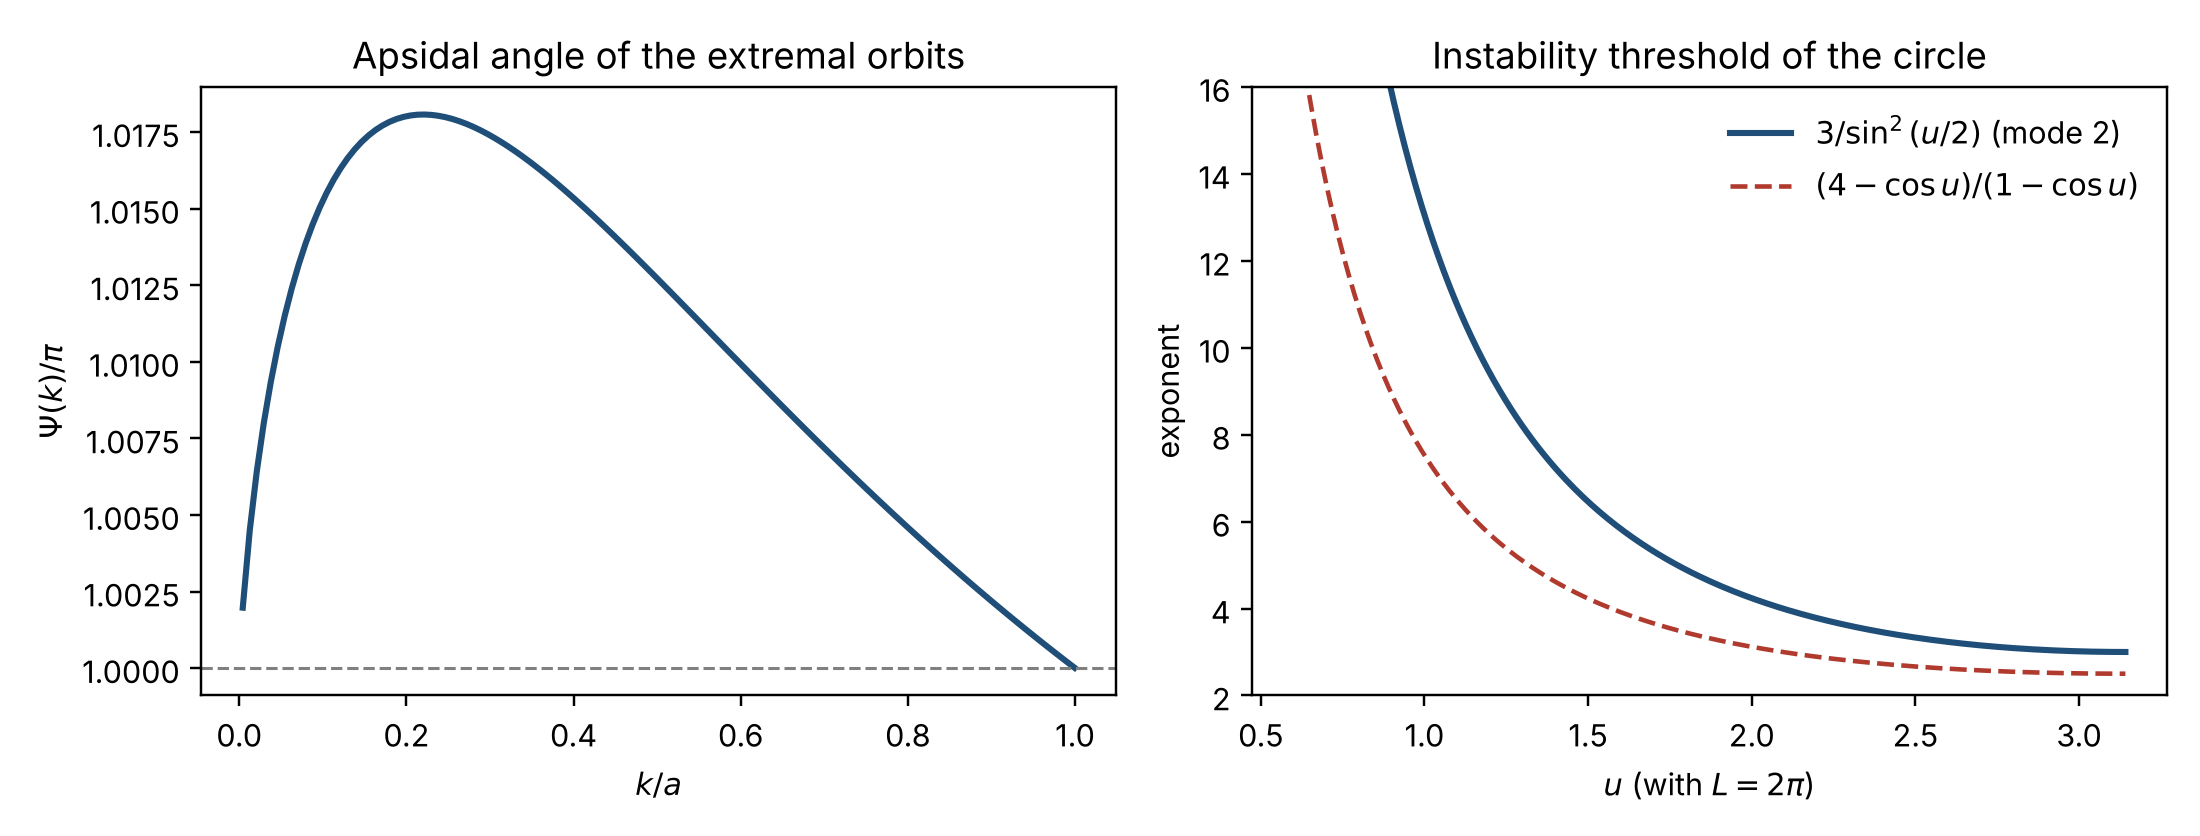
\includegraphics[width=\textwidth]{fig_apsidal.png}
\caption{Left: the apsidal angle $\Psi(k)$ of the extremal orbits, computed from \eqref{eq:TPsi}; it tends to $\pi$ at both ends and its maximum is about $1.018\pi$. Right: the exponent $3/\sin^2(u/2)$ above which the circle is unstable (Proposition~\ref{prop:mode2}) and the exponent $(4-\cos u)/(1-\cos u)$ of \cite{EFH07}, for $L=2\pi$.}
\label{fig:apsidal}
\end{figure}

\begin{remark}
Lemma~\ref{lem:apsidal} is where $p=3$ is special. For the payoff $|w|^p$ the same reduction gives $g(\rho)=\rho(E-\rho^p)$, and the apsidal angle of nearly circular orbits tends to $2\pi/\sqrt{p+1}$, which equals $\pi$ exactly when $p=3$. For $p>3$ this limit is smaller than $\pi$, and the instability of Section~\ref{sec:sharp} sets in.
\end{remark}

\section{Proof of Theorem A}\label{sec:proofA}

Let $w$ be a maximizer of $J$ on $\cA$ (Lemma~\ref{lem:exist}), and assume $J(w)>\pi^4/32$. By Lemma~\ref{lem:integrals}, its extension $W$ is a planar orbit of Section~\ref{sec:orbits} with $\lambda>0$, and $W(t+\pi)=-W(t)$. Since $|P|=E-\rho^3>0$, we have $\rho\le E^{1/3}$ and hence $J(w)\le\pi E$.

\emph{Circular orbits.} Over a time interval of length $\pi$ the angle increases by $\pi/\rho_E$, and $W(t+\pi)=-W(t)$ requires $\pi/\rho_E\in\pi+2\pi\mathbb Z$, so $\rho_E=1/(2j+1)$ with $j\ge0$. Then $J(w)=\pi\rho_E^3$, which equals $\pi$ for $j=0$ and is smaller otherwise.

\emph{Oscillating orbits.} The function $\rho$ is $\pi$-periodic with least period $T$, so $\pi=mT$ for an integer $m\ge1$. Starting at an apocentre, after time $\pi$ the point $W$ is again at an apocentre, rotated by $m\Psi$; since it equals $-W$ there, $m\Psi\in\pi+2\pi\mathbb Z$. For $m=1$ this contradicts Lemma~\ref{lem:apsidal}. Let $m\ge2$. In the normalization $E=1$, let $Q$ be a pericentre and $A$ the next apocentre. They lie at radii $\rho_1,\rho_2$ and subtend the angle $\Psi/2\in(\pi/2,3\pi/2)$ at the origin, so $\cos(\Psi/2)<0$ and
\[
\frac{T_1}2\ge|A-Q|\ge\sqrt{\rho_1^2+\rho_2^2}=\frac1{\sqrt{\rho_1+\rho_2}}\ge2^{-1/6},
\]
using $(\rho_1+\rho_2)(\rho_1^2+\rho_2^2)=1$ (Step~3) and $(\rho_1+\rho_2)^3\le2(\rho_1+\rho_2)(\rho_1^2+\rho_2^2)=2$. Hence $T_1\ge2^{5/6}$, and $\pi=mE^{1/3}T_1\ge2^{11/6}E^{1/3}$, so
\[
J(w)\le\pi E\le\pi\Bigl(\frac{\pi}{2^{11/6}}\Bigr)^3<0.69\,\pi .
\]
In every case other than the unit circle, $J(w)<\pi$. Since the maximum is at least $\pi$, it equals $\pi$, and every $w\in\cA$ with $J(w)=\pi$ is a maximizer, hence a unit circle traversed at unit speed.

By Lemma~\ref{lem:reduction} and scaling, this proves Theorem A for $p=3$, including the equality case: equality forces $|W'|=1$, so $\Gamma$ is a translate of $-W$, a circle traversed once. For $0<p<3$ Jensen's inequality gives
\[
\Bigl(\frac1L\int_0^L|\Gamma(s+L/2)-\Gamma(s)|^p\,ds\Bigr)^{1/p}\le\Bigl(\frac1L\int_0^L|\Gamma(s+L/2)-\Gamma(s)|^3\,ds\Bigr)^{1/3}\le\frac L\pi ,
\]
and equality throughout forces equality for $p=3$. The statement for $p>3$ is the case $u=L/2$ of Proposition~\ref{prop:mode2}. \qed

\section{Instability of the circle}\label{sec:sharp}

\begin{proposition}\label{prop:mode2}
Let $L=2\pi$, $0<u<2\pi$, $S=\sin^2(u/2)$, and let $\Gamma_\varepsilon$ be the closed curve with $\Gamma_\varepsilon'(s)=e^{i(s+\varepsilon\sin2s)}$. Then $\Gamma_\varepsilon$ has length $2\pi$ and, as $\varepsilon\to0$,
\[
\frac1{2\pi}\int_0^{2\pi}|\Gamma_\varepsilon(s+u)-\Gamma_\varepsilon(s)|^p\,ds=(2\sin\tfrac u2)^p\Bigl(1+\frac{pS(pS-3)}9\,\varepsilon^2+O(\varepsilon^3)\Bigr).
\]
In particular \eqref{eq:EHL} fails for small $\varepsilon\neq0$ whenever $p>3/S$.
\end{proposition}

\begin{proof}
With the Bessel expansion $e^{i\varepsilon\sin2\tau}=\sum_{k\in\mathbb Z}J_k(\varepsilon)e^{2ik\tau}$, the curve closes because only odd frequencies occur in $\Gamma'_\varepsilon$, and
\[
\Gamma_\varepsilon(s+u)-\Gamma_\varepsilon(s)=\sum_kJ_k(\varepsilon)e^{i(2k+1)s}\,\frac{e^{i(2k+1)u}-1}{i(2k+1)}=2\sin\tfrac u2\,e^{i(s+u/2)}\,F(w),
\]
where $w=e^{i(2s+u)}$, $\beta_k=\sin\frac{(2k+1)u}2\big/\bigl((2k+1)\sin\frac u2\bigr)$ and $F(w)=\sum_kJ_k(\varepsilon)\beta_kw^k$. Using $J_0=1-\frac{\varepsilon^2}4+O(\varepsilon^4)$, $J_{\pm1}=\pm\frac\varepsilon2+O(\varepsilon^3)$, $J_{\pm2}=\frac{\varepsilon^2}8+O(\varepsilon^4)$, $\beta_{-1}=1$, $\beta_{-2}=\beta_1$ and the rapid decay of $J_k$,
\[
F=1+\frac\varepsilon2(\beta_1w-\bar w)+\varepsilon^2\Bigl(-\frac14+\frac{\beta_2w^2+\beta_1\bar w^2}8\Bigr)+O(\varepsilon^3)
\]
uniformly in $w$. Writing $w=e^{i\theta}$, $|F|^2=1+X$ with
\[
X=\varepsilon(\beta_1-1)\cos\theta+\varepsilon^2\Bigl(\frac{\beta_1^2-1}4+\frac{\beta_2-\beta_1}4\cos2\theta\Bigr)+O(\varepsilon^3).
\]
Averaging over $\theta$, $\overline X=\frac{\beta_1^2-1}4\varepsilon^2+O(\varepsilon^3)$ and $\overline{X^2}=\frac{(\beta_1-1)^2}2\varepsilon^2+O(\varepsilon^3)$, so
\[
\overline{|F|^p}=1+\frac p2\overline X+\frac p4\Bigl(\frac p2-1\Bigr)\overline{X^2}+O(\varepsilon^3)
=1+\frac{p(1-\beta_1)}{16}\bigl((p-2)(1-\beta_1)-2(1+\beta_1)\bigr)\varepsilon^2+O(\varepsilon^3).
\]
Finally $\beta_1=\sin\frac{3u}2/(3\sin\frac u2)=1-\frac43S$, which gives the coefficient $pS(pS-3)/9$.
\end{proof}

For $u=\pi$ the coefficient is $p(p-3)/9$; it vanishes at $p=3$, where the circle is a degenerate but global maximizer by Theorem A. For $p=2$ and every $u$ it equals $-\frac{2S(3-2S)}9<0$, as Lük\H{o}'s inequality requires.

\section*{Declarations}

\noindent\textbf{Funding.} This research received no external funding.

\noindent\textbf{Conflict of interest.} The author declares no conflict of interest.

\noindent\textbf{Data availability.} No data were generated. The figure is computed from the integrals \eqref{eq:TPsi}. Scripts checking the algebra of Section~5 and the numerics are archived at \url{https://doi.org/10.5281/zenodo.24128091}.

\noindent\textbf{Acknowledgements.} The problem and its physical motivation are due to P.~Exner, E.~M.~Harrell and M.~Loss; the case $p=2$ is due to G.~Lük\H{o}. The proof uses the maximum principle of L.~S.~Pontryagin and his collaborators.

\begin{thebibliography}{99}

\bibitem{ACFGH03} A.~Abrams, J.~Cantarella, J.~H.~G.~Fu, M.~Ghomi and R.~Howard, \emph{Circles minimize most knot energies}, Topology \textbf{42} (2003), 381--394, \doi{10.1016/S0040-9383(02)00016-2}.

\bibitem{Arn89} V.~I.~Arnold, \emph{Mathematical Methods of Classical Mechanics}, 2nd ed., Graduate Texts in Mathematics \textbf{60}, Springer, New York, 1989, \doi{10.1007/978-1-4757-2063-1}.

\bibitem{EFH07} P.~Exner, M.~Fraas and E.~M.~Harrell, \emph{On the critical exponent in an isoperimetric inequality for chords}, Phys. Lett. A \textbf{368} (2007), 1--6, \doi{10.1016/j.physleta.2007.03.067}.

\bibitem{Exn05} P.~Exner, \emph{An isoperimetric problem for leaky loops and related mean-chord inequalities}, J. Math. Phys. \textbf{46} (2005), 062105, \doi{10.1063/1.1914728}.

\bibitem{Exn08} P.~Exner, \emph{Leaky quantum graphs: a review}, in: Analysis on Graphs and its Applications, Proc. Sympos. Pure Math. \textbf{77}, Amer. Math. Soc., Providence, RI, 2008, 523--564, \doi{10.1090/pspum/077/2459890}.

\bibitem{EHL06} P.~Exner, E.~M.~Harrell and M.~Loss, \emph{Inequalities for means of chords, with application to isoperimetric problems}, Lett. Math. Phys. \textbf{75} (2006), 225--233, \doi{10.1007/s11005-006-0053-y}.

\bibitem{EHL06a} P.~Exner, E.~M.~Harrell and M.~Loss, \emph{Addendum to: Inequalities for means of chords, with application to isoperimetric problems}, Lett. Math. Phys. \textbf{77} (2006), 219, \doi{10.1007/s11005-006-0087-1}.

\bibitem{Luk66} G.~Lük\H{o}, \emph{On the mean length of the chords of a closed curve}, Israel J. Math. \textbf{4} (1966), 23--32, \doi{10.1007/BF02760067}.

\bibitem{Pec92} P.~Pech, \emph{Chords and arclength of a closed space curve}, Czechoslovak Math. J. \textbf{42} (1992), 471--474, \doi{10.21136/CMJ.1992.128343}.

\bibitem{PBGM62} L.~S.~Pontryagin, V.~G.~Boltyanskii, R.~V.~Gamkrelidze and E.~F.~Mishchenko, \emph{The Mathematical Theory of Optimal Processes}, Interscience, New York, 1962.

\end{thebibliography}

\end{document}
